\chapter{Implementierung}
\label{chapter5}

Wie bereits erwähnt erfolgte die Implementierung in Java.
Damit für die Nutzung keine weiteren Installationen nötig sind,
wurden nur die Standardbibliotheken zur Umsetzung genutzt.
Der gesamte Source Code kann unter \href{https://github.com/lzfs/tsprocessor}{github/lzfs/tsprocessor}
abgerufen werden.
In diesem Kapitel wird vertiefend auf die Struktur des Tools eingegangen
und wichtige Aspekte der Implementierung betrachtet.


\section{Aufbau}
\label{5-Aufbau}
Der detailierte Aufbau des Tools kann \autoref{fig:Classes} entnommen werden.
Hier wurde aus Gründen der Übersichtlichkeit auf Konstruktoren,
sowie Getter- und Setter-Methoden verzichtet.
Die Architektur wird im Folgenden detailiert beschrieben.

\begin{figure}[ht]
    \begin{center}
        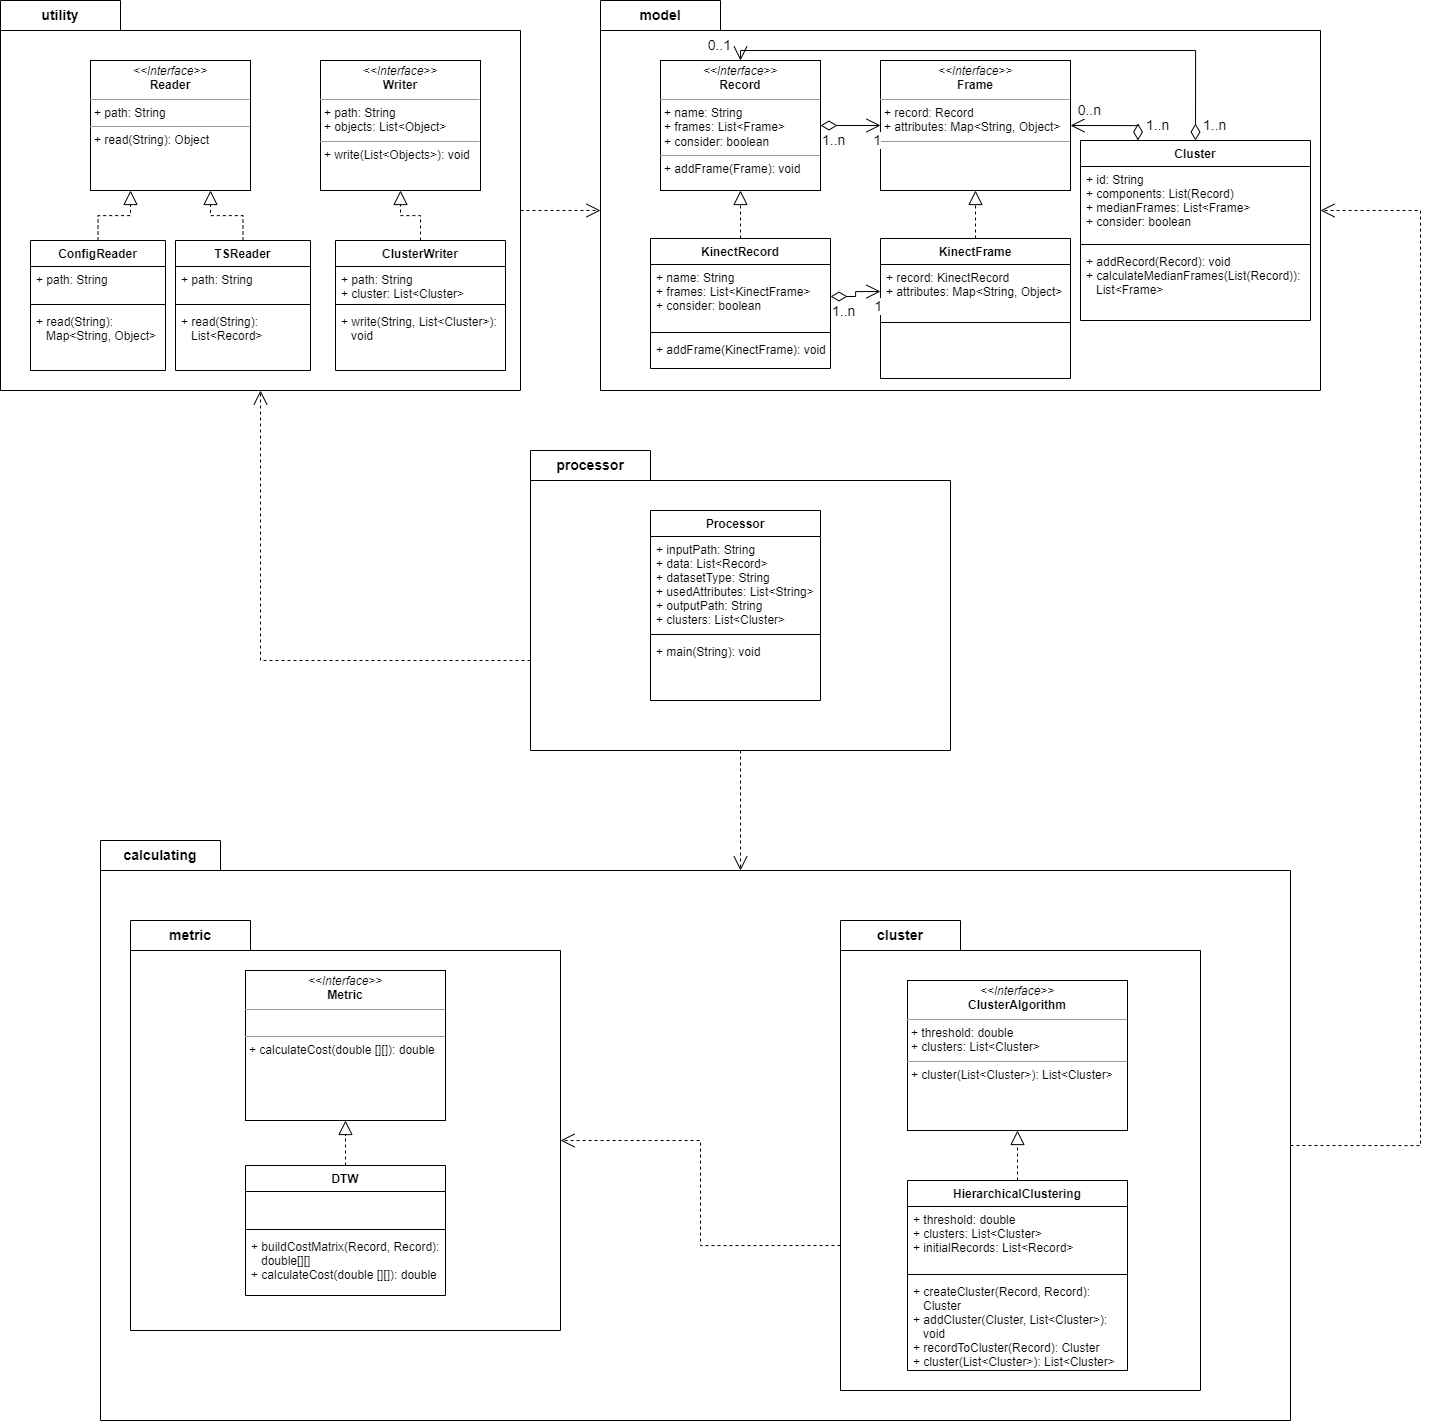
\includegraphics[width=0.7\textwidth]{classes.png}
    \end{center}
    \caption{Klassendiagramm des Tools.}
    \label{fig:Classes}
\end{figure}



\section{Codebeschreibung}
\label{5-Codebeschreibung}

\begin{lstlisting}[language=Java, caption=Processor-Workflow.]
    if (datasetType.equals("kinect")) {
            DataReader dataReader
                = new DataReader(
                    "D:",
                    separator,
                    attributes);
            data = dataReader.read(inputPath);

            HierarchicalClustering clustering
                = new HierarchicalClustering(
                    data,
                    threshold,
                    attributes,
                    usedAttributes,
                    distanceFunction);
            clusterImpls = clustering.cluster();

            ClusterWriter writer = new ClusterWriter();
            writer.write(
                outputPath,
                clusterImpls);

            VisualizerImpl visualizerImpl
                = new VisualizerImpl(
                    flipVisualization,
                    bodyIdParamName);
            for (ClusterImpl clusterImpl : clusterImpls) {
                visualizerImpl.visualize(
                    clusterImpl.getId(),
                    outputPath,
                    clusterImpl.getMedianFrames());
            }
        }
\end{lstlisting}


\begin{lstlisting}[language=Java, caption=Berechnung der Kosten.]
    public double calculateCost(
        List<FrameImpl> frames1,
        List<FrameImpl> frames2) {
        // add the calculated cost of each attribute to it
        double cost = 0;
        // calculate the cost for all attributes
        for (String attribute : this.usedAttributes) {
            // build the cost matrix for this attribute
            double[][] dtwMatrix = buildCostMatrix(
                frames1,
                frames2,
                attribute);
            // calculate and add the cost of this attribute
            cost += calculatePathCost(dtwMatrix);
        }
        return cost / this.usedAttributes.size();
    }
\end{lstlisting}


\begin{lstlisting}[language=Java, caption=Kostenmatrix.]
    private double[][] buildCostMatrix(
        List<FrameImpl> frames1,
        List<FrameImpl> frames2,
        String attribute) {
        double[] s = new double[frames1.size()];
        double[] t = new double[frames2.size()];

        int counter = 0;
        for (FrameImpl frame : frames1) {
            s[counter] = Double.parseDouble(frame.getValue(attribute));
            counter += 1;
        }
        counter = 0;
        for (FrameImpl frame : frames2) {
            t[counter] = Double.parseDouble(frame.getValue(attribute));
            counter += 1;
        }

        int n = s.length;
        int m = t.length;
        // filled with zeros by default
        double[][] dtwMatrix = new double[n + 1][m + 1];

        for (int i = 0; i < dtwMatrix.length; i++) {
            for (int j = 0; j < dtwMatrix[0].length; j++) {
                // filled with infinity by definition of dtw
                dtwMatrix[i][j] = Double.POSITIVE_INFINITY;
            }
        }
        // filled with 0 by definition of dtw
        dtwMatrix[0][0] = 0;

        for (int i = 1; i < dtwMatrix.length; i++) {
            for (int j = 1; j < dtwMatrix[0].length; j++) {
                // this is the default distance function
                double cost = Math.abs(s[i - 1] - t[j - 1]);
                
                double minTmp = Math.min(
                    dtwMatrix[i - 1][j],
                    dtwMatrix[i][j - 1]);
                double lastMin = Math.min(
                    minTmp,
                     dtwMatrix[i - 1][j - 1]);
                dtwMatrix[i][j] = cost + lastMin;
            }
        }
        return dtwMatrix;
    }
\end{lstlisting}

\begin{lstlisting}[language=Java, caption=Warping Path berechnen.]
    public double calculatePathCost(double[][] dtwMatrix) {
        int n = dtwMatrix.length - 1;
        int m = dtwMatrix[n - 1].length - 1;
        int pathCounter = 1;
        double cost = dtwMatrix[n][m];
        while (n != 0 && m != 0) {
            // dynamic time warping algorithm
            double minTmp = Math.min(dtwMatrix[n - 1][m], dtwMatrix[n][m - 1]);
            double lastMin = Math.min(minTmp, dtwMatrix[n - 1][m - 1]);
            cost += lastMin;
            if (lastMin == dtwMatrix[n - 1][m - 1]) {
                n = n - 1;
                m = m - 1;
            }
            else if (lastMin == dtwMatrix[n - 1][m]) {
                n = n - 1;
            }
            else if (lastMin == dtwMatrix[n][m - 1]) {
                m = m - 1;
            }
            pathCounter += 1;
        }
        return cost / pathCounter;
    }
\end{lstlisting}

\begin{lstlisting}[language=Java, caption=Hierarchisches Clustering.]
    public List<ClusterImpl> cluster() {
        List<ClusterImpl> result = new ArrayList<>();
        // initialize each record as a cluster and add it to the clusters list
        for (RecordImpl record : this.initialRecords) {
            this.clusterImpls.add(this.recordToCluster(record));
        }
        double currentMinimumCost;
        double cost;
        int mergeCandidate1;
        int mergeCandidate2;

        do {
            // reset for next loop iteration
            currentMinimumCost = this.dtw.calculateCost(    
                this.clusterImpls.get(0).getMedianFrames(),
                this.clusterImpls.get(1).getMedianFrames());
            cost = this.dtw.calculateCost(  
                this.clusterImpls.get(0).getMedianFrames(),
                this.clusterImpls.get(1).getMedianFrames());
            mergeCandidate1 = 0;
            mergeCandidate2 = 1;
            for (ClusterImpl clusterImpl1 : this.clusterImpls) {
                for (ClusterImpl clusterImpl2 : this.clusterImpls) {
                    if (
                        clusterImpl1 != clusterImpl2
                        && clusterImpl1.isConsider()
                        && clusterImpl2.isConsider()) {
                        if (this.calculatedCost.containsKey(
                            new ClusterKey(
                                clusterImpl1,
                                clusterImpl2))) {
                            cost = this.calculatedCost.get(
                                new ClusterKey(
                                    clusterImpl1,
                                    clusterImpl2));
                        }
                        else {
                            cost = this.dtw.calculateCost(
                                clusterImpl1.getMedianFrames(),
                                clusterImpl2.getMedianFrames());
                            this.calculatedCost.put(
                                new ClusterKey(
                                    clusterImpl1,
                                    clusterImpl2),
                                cost);
                        }
                        if (cost <= currentMinimumCost) {
                            /* if a cost smaller than the current minimum cost
                            is found this will be the new cost */
                            currentMinimumCost = cost;
                            mergeCandidate1 =
                                this.clusterImpls.indexOf(clusterImpl1);
                            mergeCandidate2 =
                                this.clusterImpls.indexOf(clusterImpl2);
                        }
                    }
                }
            }
            // if the minimum cost is still below the threshold we can continue
            if (
                currentMinimumCost < threshold
                && currentMinimumCost > this.minConst) {
                /* Combining mergeCandidate1 and mergeCandidate2
                has the lowest found cost.
                These two should therefore be merged together.
                Merge cluster2 into cluster1 and update the cluster list.
                Consider of cluster2 is set to false. */
                this.clusterImpls.get(mergeCandidate1).mergeWithCluster(
                    this.clusterImpls.get(mergeCandidate2));

                // create a copy of the map to avoid an exception
                Map<ClusterKey, Double> calculatedCostCopy = new HashMap<>();
                calculatedCostCopy.putAll(calculatedCost);

                /* remove all calculated costs from the map that contain
                cluster1 because it changed and therefore all cost values
                with this cluster have to be calculated again */
                for (Map.Entry<ClusterKey, Double> entry : calculatedCostCopy.entrySet()) {
                    /* ignore mergeCandidate2 because the consider
                    value of cluster2 is set to false */
                    if (entry.getKey().getCluster1().getId() == mergeCandidate1) {
                        for (ClusterImpl clusterImpl : clusterImpls) {
                            calculatedCost.remove(
                                new ClusterKey(
                                    this.clusterImpls.get(mergeCandidate1),
                                    clusterImpl));
                        }
                    }
                }
            }
        } while (
            currentMinimumCost < threshold
            && currentMinimumCost > this.minConst);
        /* clean up the list of found clusters by removing all clusters
        that shouldn't be considered anymore */
        for (ClusterImpl clusterImpl : this.clusterImpls) {
            if (clusterImpl.isConsider()) {
                result.add(clusterImpl);
            }
        }
        return result;
    }
\end{lstlisting}

\section{Abweichungen zur Konzeption}
\label{5-AbweichungenKonzeption}

\section{Verbesserung der Performanz}
\label{5-Performanz}
